\documentclass[12pt]{article}
\usepackage[utf8]{inputenc}
\usepackage[T1]{fontenc}
\usepackage[polish]{babel}
\usepackage{geometry}
\usepackage{tabularx}
\usepackage[table,xcdraw,dvipsnames]{xcolor}
\usepackage{color}
\usepackage{subfig}
\usepackage{sidecap}
\usepackage{wrapfig}
\usepackage{float}
\usepackage{enumerate}
\usepackage{graphicx}
\usepackage{multirow}
\setlength{\parindent}{0pt}
\usepackage{hyperref}
\usepackage{titlesec}
\titlelabel{\thetitle.\quad}
\usepackage{amsmath}
\usepackage{anyfontsize}
\usepackage{indentfirst}
\usepackage{listings}
\usepackage{multicol}
\usepackage{pgfplots}
\usepackage{listings}
\newgeometry{tmargin=1.8cm,bmargin=1.8cm,lmargin =1.8cm,rmargin=1.8cm}

\begin{document}
    
\begin{titlepage}
    \begin{figure}
        \centering
        
\includegraphics[width=18cm]{logo-PWr.png}
        
        \label{fig:pwr}
    \end{figure}
        \begin{center}
            \huge Wydział Elektroniki, Fotoniki i Mikrosystemów \\ 
            \vspace{40pt}
            \huge Projektowanie algorytmów i metody sztucznej inteligencji  \\
        \end{center}
        \vspace{60pt}
        \hrule
        \vspace{1pt}
        \hrule
        \begin{center}
            {\fontsize{40}{50}\selectfont Projekt 1\\ }
            \vspace{10pt}
            {\fontsize{25}{25}\selectfont Zadanie na ocenę bdb }
        \end{center}
        \hrule
        \vspace{1pt}
        \hrule
        \begin{flushright}
            \vspace{65pt}
            \textit{\Large Prowadzący:}\\
            
            \Large Dr inż. Łukasz Jeleń\\
            \vspace{10pt}
            \textit{\Large Wykonała:}\\
            \Large Zuzanna Mejer, 259382 \\
        
        \end{flushright}
        \vspace{65pt}
        \begin{center}
            \large Wrocław, \today r.
        \end{center}
    \end{titlepage}

\section{Wstępne założenia}
Zadanie polegało na zaprojektowaniu i zaimplementowaniu algorytmu, który radziłby sobie z sortowaniem otrzymanych 
pakietów składających się z numeru i tekstu wiadomości. Do wykonania zadania przyjęto pewne założenia. 
Pierwszym z nich jest przyjęcie perspektywy Anny i jej komputera. Oznacza to tyle, że napisany program nie zajmuje się 
dzieleniem wiadomości na \textit{n} pakietów oraz nie nadaje im numerów, gdyż wymienione czynności wykonywał,
zgodnie z poleceniem, Jan na swoim komputerze. Zatem program został przygotowany tak, żeby pracować już z 
losowo ułożonymi i ponumerowanymi pakietami. Drugim przyjętym założeniem jest przesyłanie tych pakietów w jednym 
pliku tekstowym jako drugi argument wywołania podczas uruchamiania pliku wykonywalnego. Kolejnym założeniem jest
forma zakończenia programu i wyświetlenie posortowanej wiadomości. Zdecydowano, że posortowana wiadomość
nie tylko będzie wyświetlana na standardowym wyjściu, ale również będzie zapisywana do nowo 
tworzonego pliku nazwanego ,,uporządkowany\_list.txt''. 

\section{Struktura danych}
W celu zrealizowania zadania wybrano strukturę danych do przechowywania informacji (numeru i tekstu wiadomości), 
jaką jest kolejka priorytetowa na bazie listy dwukierunkowej. Poniżej przedstawiono uzasadnienie wyboru.
Kolejka priorytetowa jest abstrakcyjnym typem danych, służącym do przechowywania 
zbioru elementów, przy czym każdy element posiada dodatkowe pole do przechowywania priorytetu 
(klucza). Zatem, z założenia, do kolejki priorytetowej można wprowadzać pakiety, składające się 
z numeru (priorytetu) i tekstu. Kolejnym argumentem przemawiającym za użyciem kolejki priorytetowej 
jest układanie elementów w kolejce kolejności priorytetu rosnąco. Lista dwukierunkowa umożliwia wstawianie elementu 
w dowolnym miejscu, nie tylko na początku lub na końcu listy, co pozwala na wydajne sortowanie elementów przy ich 
wstawianiu do kolejki. Analogicznie, lista dwukierunkowa pozwala także na 
usuwanie elementów z dowolnego miejsca.

\section{Omówienie programu}
\subsection{Obsługa plików}
Do obsługi plików została stworzona klasa o nazwie \textit{file} z dwoma prywatnymi polami 
określającymi plik wejściowy \textit{in\_file} oraz plik wyjściowy \textit{out\_file}.
Stworzone zostały metody służące do otwierania i zamykania plików wejściowych i wyjściowych 
(\textit{open\_in\_file, open\_out\_file, close\_in\_file, close\_out\_file}), 
czytania (\textit{read\_file}) i sprawdzania końca (\textit{end\_of\_file}) pliku wejściowego
oraz zapisywania do pliku wyjściowego (\textit{write\_out\_file}).

\lstset{language=C++, firstnumber=1, keywordstyle=\color{blue}, numbers=left, frame = single}
\begin{lstlisting}
#ifndef OBSLUGA_PLIKOW.HH
#define OBSLUGA_PLIKOW.HH

#include <iostream>
#include <string>
#include <fstream>

class file
{
    private:
        std::fstream in_file;
        std::fstream out_file;

    public:
        void open_in_file(std::string name_file);
        void open_out_file(std::string name_file);
        void read_file(int &key, std::string &text);
        void write_out_file(const std::string &text);
        void close_in_file();
        void close_out_file();
        bool end_of_file();
};
#endif
\end{lstlisting}

Plik wejściowy podawany przy uruchomieniu programu ma domyślnie formę przedstawioną 
na poniższym zdjęciu. Na początku linii jest numer pakietu, a po spacji wiadomość. 

\begin{figure}[H]
    \centering
    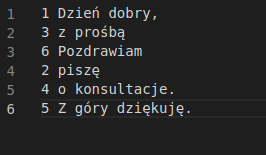
\includegraphics[width=7cm]{format_pliku.png}
    \caption{Format pliku wejściowego}
    \label{fig: format_plku}
\end{figure}


\subsection{Kolejka priorytetowa jako lista dwukierunkowa}
Do zaimplementowania kolejki na liście dwukierunkowej, została stworzona struktura \textit{node}, 
która ma dwa pola do przechowywania pakietu: \textit{key} oraz \textit{text}, oraz dwa wskaźniki 
na następny i poprzedni element: \textit{*next} i \textit{*prev}. Została stworzona klasa 
\textit{priority\_queue} z pierwszym wskaźnikiem na początek kolejki: \textit{*header} 
typu struktury \textit{node}. Zostały zaimplementowane metody:
\begin{itemize}
    \item \textit{comparison} - służy do porównywania wartości dwóch kluczy i jest 
    wykorzystywana przy sortowaniu elementów podczas wprowadzania do kolejki.
    \item \textit{insert} - odpowiednik metody \textit{push}; służy do wstawiania elementów 
    do kolejki w dowolnym miejscu w kolejce, tak, aby tworzyć kolejkę uporządkowaną rosnąco. 
    \item \textit{display\_text} - odpowiednik metody \textit{top}; odpowiada za
    wyświetlanie samego tekstu pierwszego elementu w kolejce.
    \item \textit{remove\_minimum} - odpowiednik \textit{pop}; służy do usuwania elementu z 
    początku kolejki. 
    \item \textit{empty} - zwraca informację o tym, czy kolejka jest pusta.
    \item \textit{return\_minimum} - jest funkcją pomocniczą do zwracania tekstu pierwszego 
    elementu w kolejce. Wykorzystuje ją metoda zapisywania do pliku. 
    \item \textit{size} - zwraca ilość elementów umieszczonych w kolejce priorytetowej.
\end{itemize}

\lstset{language=C++, firstnumber=1, keywordstyle=\color{blue}, numbers=left, frame = single}
\begin{lstlisting}
#ifndef PRIORITY_QUEUE.HH
#define PRIORITY_QUEUE.HH
#include <iostream>

struct node
{
    int key;
    std::string text;
    node *prev = nullptr;
    node *next = nullptr;
};

class priority_queue
{

private:
    node *header = nullptr;
    bool comparison(int x, int y);

public:
    void insert(int key, std::string text);
    void display_text();
    void remove_minimum(); 
    bool empty();
    std::string return_minimum();
    int size();
};
#endif
\end{lstlisting}

\subsection{Działanie programu}
Program wykonuje następujące działania:
\begin{enumerate}
    \item Otwiera zarówno plik wejściowy, podany jako argument wywołania pliku wykonywalnego, 
    jak i wyjściowy, do którego będą zapisywane dane.
    \item Aż do natrafienia na koniec danych w pliku, program sczytuje kolejne sekwencje, 
    tworzy nowy element typu \textit{node}, przypisuje do niego wartości klucza i wiadomości,
    a następnie wstawia w odpowiednie miejsce w kolejce, sortując rosnąco względem wartości klucza.  
    \item Kiedy nie ma więcej danych w pliku i kolejka jest już utworzona, następuje wyświetlenie
    tekstu elementu o najmniejszej wartości klucza na standardowe wyjście, zapisanie go do pliku 
    wyjściowego oraz usunięcie go z kolejki priorytetowej. Ten etap powtarza się aż do wyczyszczenia 
    całej kolejki.   
\end{enumerate}

\lstset{language=C++, firstnumber=1, keywordstyle=\color{blue}, numbers=left, frame = single}
\begin{lstlisting}
    #include "obsluga_plikow.hh"
    #include "priority_queue.hh"
    #include <iostream>
    
    int main(int argc, char *argv[])
    {
      priority_queue kolejka;
      file plik;
      int klucz;
      std::string tekst;
      plik.open_in_file(argv[1]);
      plik.open_out_file("uporzadkowany_list");
    
      while (!plik.end_of_file())
      {
        plik.read_file(klucz, tekst);
        kolejka.insert(klucz, tekst);
      }
      
      while(!kolejka.empty())
      {
        kolejka.display_text();
        plik.write_out_file(kolejka.return_minimum());
        kolejka.remove_minimum();
      }
      std::cout << "\n";
    
      plik.close_in_file();
      plik.close_out_file();
    }
\end{lstlisting}


\section{Analiza złożoności obliczeniowej}
Najbardziej znaczące metody do badania złożoności obliczeniowej programu to metody 
\textit{insert} oraz \textit{remove\_minimum}. Ze względu na zastosowanie implementacji 
na liście posortowanej, można się spodziewać, że złożoność obliczeniowa metody 
\textit{insert} będzie równa \textit{O(n)}, co oznaczałoby, że czas potrzebny do wykonania 
się tej metody będzie liniowo zależny od liczby elementów w pliku.
Z kolei złożoność obliczeniowa metody \textit{remove\_minimum} powinna wynosić \textit{O(1)}, 
co oznaczałoby, że metoda ta jest stała w czasie - niezależna od liczby elementów w kolejce.

Przeprowadzono testy, które miały potwierdzić lub odrzucić przedstawioną hipotezę.
W tym celu wykorzystano bibliotekę \textit{chrono} i funkcję \textit{clock}.
Zmierzono zależność czasu w nanosekundach od liczby elementów (ograniczając się 
do 10 000 elementów). W przypadku badania metody \textit{insert}, wykorzystano najgorszy przypadek,
to znaczy, że w pliku wejściowym wartości kluczy były zapisane rosnąco, tak, aby metoda za każdym razem dodawała 
na koniec kolejki - wykonywała najwięcej przesunięć. Poniżej przedstawiono wykresy badanych zależności:

\begin{figure}[H]
    \centering
    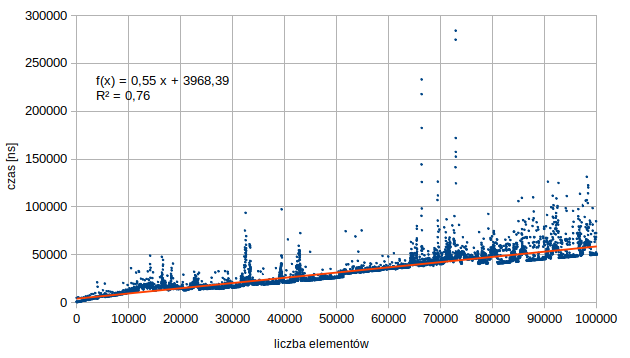
\includegraphics[width=15cm]{O_insert.png}
    \caption{Zależność czasu działania metody \textit{insert} od liczby elementów w kolejce}
    \label{fig: O_insert}
\end{figure}

\begin{figure}[H]
    \centering
    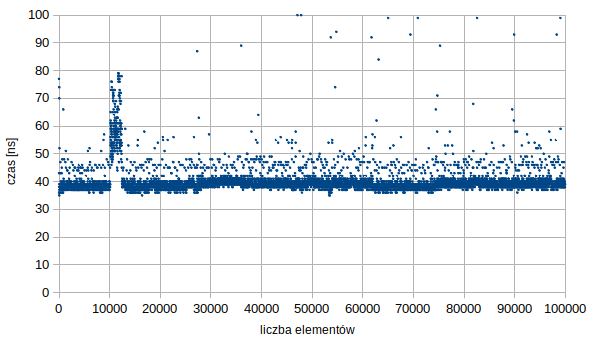
\includegraphics[width=15cm]{O_remove.png}
    \caption{Zależność czasu działania metody \textit{remove\_minimum} od liczby elementów w kolejce}
    \label{fig: O_remove}
\end{figure}

Pomimo dużych odchyleń, można zauważyć, że wykresy potwierdziły hipotezę - metoda \textit{insert} ma złożoność obliczeniową 
liniową \textit{O(n)}, a metoda \textit{remove\_minimum} ma złożoność obliczeniową stałą w czasie 
\textit{O(1)}.

\section{Podsumowanie i wnioski}
\begin{itemize}
    \item Dobór struktury danych okazał się być dobry. Lista dwukierunkowa bardzo usprawniła działanie programu i 
    efektywność metod.
    \item Lista uporządkowana sprawiła, że złożoność obliczeniowa metody \textit{insert} oraz \textit{remove\_minimum}
    wyniosła kolejno \textit{O(n)} oraz \textit{O(1)}. Zastosowanie listy nieuporządkowanej nie zmieniłoby ogólnej 
    złożoności obliczeniowej programu. 
    \item Można powiedzieć, że złożoność obliczeniowa programu jest funkcją liniową. Jest to dobry wynik, lecz dla 
    dużej ilości danych lepsza byłaby złożoność w funkcji logarytmicznej.
\end{itemize}


\section{Literatura}
\begin{enumerate}
    \footnotesize
    \item Wykład ,,Projektowanie Algorytmów i Metody Sztucznej Inteligencji''
    \item M.T.Goodrich, R. Tamassia, D.Mount ,,Data Structures \& Algorithms in C++''
    \item \url{ https://cpp0x.pl/kursy/Kurs-STL-C++/Adapter-kolejki-priorytetowej-std-priority_queue/118} (dostęp: 31.03.2022)
\end{enumerate}

\end{document}